\documentclass{article}
\usepackage[utf8]{inputenc}
\usepackage[T1]{fontenc}
\usepackage[utf8]{inputenc}
\usepackage[norsk]{babel}
\usepackage{amsmath}
\usepackage{hyperref}
\usepackage{enumerate}
\usepackage{graphicx}
\usepackage{listings}
\usepackage{color}
\usepackage{gensymb}
\usepackage{subfig}
\usepackage{fancyvrb}
\definecolor{codegreen}{rgb}{0,0.6,0}
\definecolor{codegray}{rgb}{0.5,0.5,0.5}
\definecolor{codepurple}{rgb}{0.58,0,0.82}
\definecolor{backcolour}{rgb}{0.95,0.95,0.92}
\setlength{\parindent}{0pt}
\lstdefinestyle{mystyle}{
    backgroundcolor=\color{backcolour},
    commentstyle=\color{codegreen},
    keywordstyle=\color{magenta},
    numberstyle=\tiny\color{codegray},
    stringstyle=\color{codepurple},
    basicstyle=\footnotesize,
    breakatwhitespace=false,
    breaklines=true,
    captionpos=b,
    keepspaces=true,
    numbers=left,
    numbersep=5pt,
    showspaces=false,
    showstringspaces=false,
    showtabs=false,
tabsize=2}
\lstset{style=mystyle}

\title{Oblig1 INF4300}
\author{mathiaki}


\begin{document}

\maketitle

\newpage
\tableofcontents
\newpage

\section{Texture description}
In this part of the report I will try to analyze the different textures.
I will go through every sub-texture and give a description based on: characteristics, texture direction, frequency of the texture, variance of the texture, homogeneity, and the size of the texture elements.  \\

 
Before i describe the different textures, i will index the different images in the following way: (the same is true for the program)\\
\begin{figure}[h]

\centering
\begin{BVerbatim}
 img0        img1      img0     img1
|---|---| |---|---| |-------| |-------|
| 0 | 1 | | 4 | 5 | |       | |       |
|---|---| |---|---| |   8   | |   9   |
| 2 | 3 | | 6 | 7 | |       | |       |
|---|---| |---|---| |-------| |-------|

\end{BVerbatim}
\caption{Order of analyze}%
\label{verb:comp}
\end{figure}


This means i will start in the top left corner of mosaic1 and and in the bottom right corner of mosaic2. \\
\textit{In the program 8 and 9 is reserved for the whole mosaic1 and mosaic2 respectively.} 

\newpage
\setcounter{subsection}{-1}
\subsection{Texture 0}
\textbf{Characteristics:}\\
Texture is mainly random noise. Somewhere in the texture you get some patters that looks like holes. \\

\textbf{Texture Direction}\\
There are a slight movement in the $\frac{3\pi}{4}$ rad direction, and as mentioned, some circular patterns can be observed. \\

\textbf{Frequency} \\
The crevasses is on a rough average 10px in diameter, and the edges between them is closer to 4px.\\ 


\textbf{Variance}\\
If we look at the histogram, we can see that it is one of the textures with the least variance. We do have some peaks int the histogram that drives down the variance a bit\\

\textbf{Homogeneity}\\
The texture is has very few homogeneous areas.\\

\textbf{Texture element size}\\
As mentioned, the texture is very similar to random noise, so the size is hard to determine. If we think of the elements as the crevasses, the texture element size is a few pixels.  

\begin{figure}[h]%
	\centering
    \subfloat[Texture 0]{{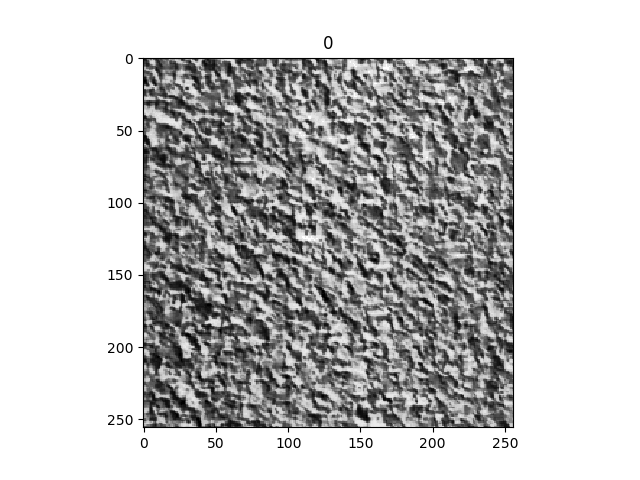
\includegraphics[width=5.5cm]{0.png} }}%
    \qquad
    \subfloat[Histogram of Texture 0 0]{{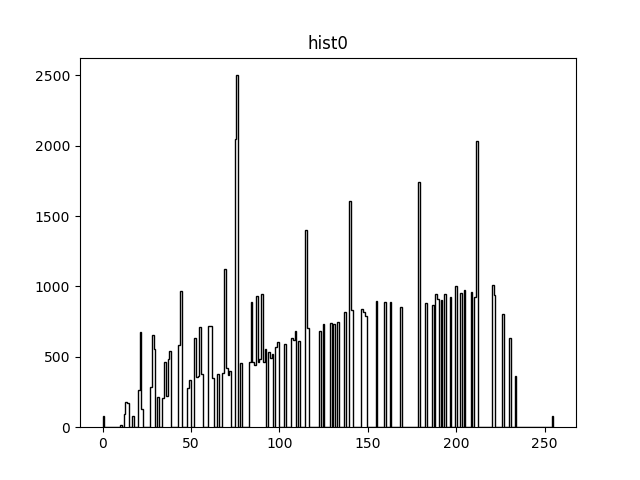
\includegraphics[width=5.5cm]{hist0.png} }}%
    \caption{Texture with histogram}%
    \label{fig:IMG0}%
\end{figure}



\newpage
\subsection{Texture 1}
\textbf{Characteristics:}\\
Texture has a clearer pattern of squares that is roughly 8 px wide and high.
It is also some random noise in the top left corner of the texture. 
\\

\textbf{Texture Direction}\\
The texture direction is almost horizontal (and vertical), with a slight angle clockwise.\\

\textbf{Frequency} \\
The frequency of the squares are approximately 1/40. Since there are that many repetitions in the image. 
\\ 


\textbf{Variance}\\
The histogram is fairly balanced, so the variance is in the middle if the spectrum. Especially compared to \ref{fig:IMG2} \\

\textbf{Homogeneity}\\
The texture is has no big homogeneous areas.\\


\textbf{Texture element size}\\
As mentioned, the squares has a diameter of approximatively 7 px.



\begin{figure}[h]%
	\centering
    \subfloat[Texture 1]{{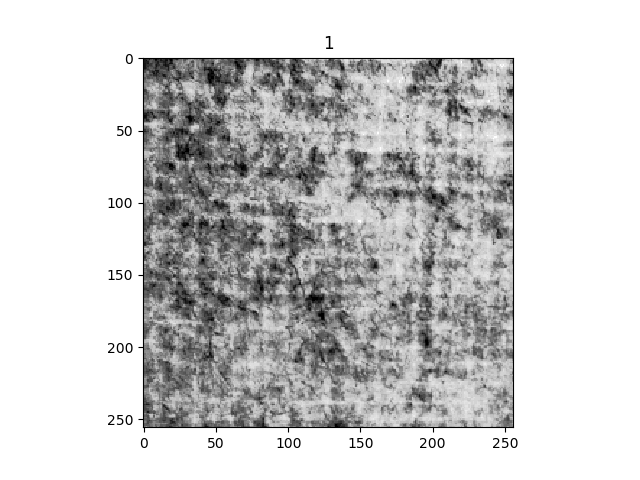
\includegraphics[width=5.5cm]{1.png} }}%
    \qquad
    \subfloat[Histogram of Texture 1]{{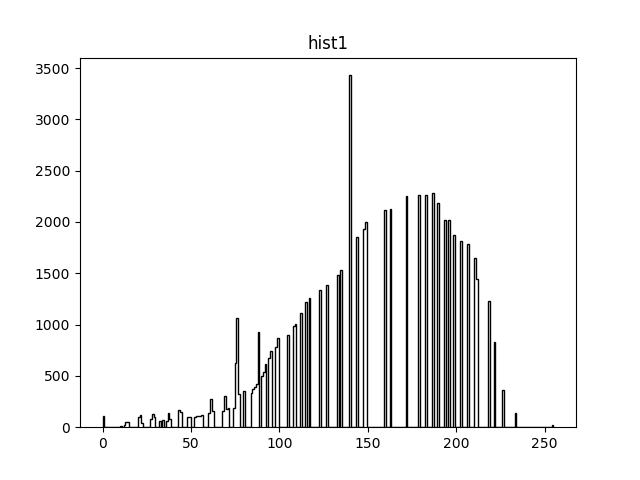
\includegraphics[width=5.5cm]{hist1.png} }}%
    \caption{Texture with histogram}%
    \label{fig:IMG1}%
\end{figure}





\newpage
\subsection{Texture 2}
\textbf{Characteristics:}\\
The texture is a series of lines that face in roughly the same direction.
\\

\textbf{Texture Direction}\\
The majority of the stripes has an angle of 100$\degree$. (or 1.745 rad)\\ 
 
\textbf{Frequency} \\
The frequency of the pattern, diagonally to the lines is 3-4 pixels in width, and they are repeating 30-40 times in the picture.
\\ 


\textbf{Variance}\\
This pattern has a small variance, probably the smallest.
\\

\textbf{Homogeneity}\\
The texture has large homogeneous areas, both in and around the stripes.\\

\textbf{Texture element size}\\
The element size is only a few pixels wide, and around 50 pixels high.


\begin{figure}[h]%
	\centering
    \subfloat[Texture 2]{{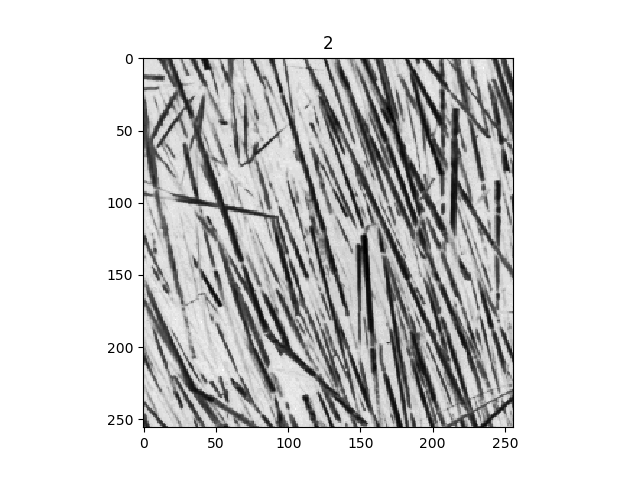
\includegraphics[width=5.5cm]{2.png} }}%
    \qquad
    \subfloat[Histogram of Texture 2]{{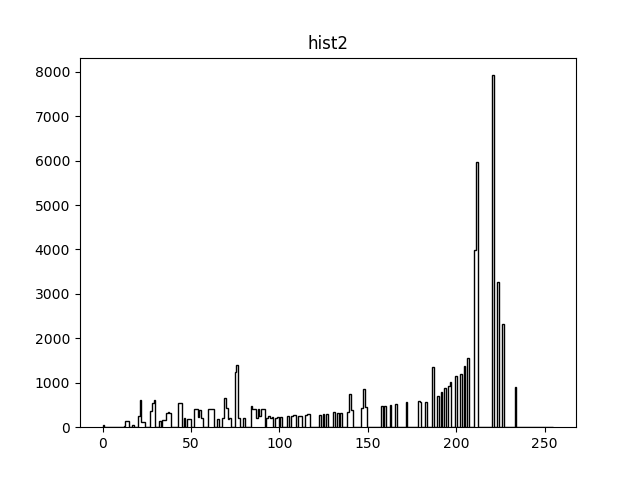
\includegraphics[width=5.5cm]{hist2.png} }}%
    \caption{Texture with histogram}%
    \label{fig:IMG2}%
\end{figure}





\newpage
\subsection{Texture 3}
\textbf{Characteristics:}\\
This seems like another white noise texture. Difference between this and \ref{fig:IMG0} is that the first image had crevasses, and this does not. \\

\textbf{Texture Direction}\\
There are no clear direction in the texture. This (and partly \ref{fig:IMG0}) is isotropic textures.
\\ 
 
\textbf{Frequency} \\
It is hard to say anything about the frequency, but a rough guess might be 2-3px of the same grey-scale. This means a high frequency\\ 


\textbf{Variance}\\
This pattern has a low variance, but the pixel value aprox. 75 upping the variance.
\\

\textbf{Homogeneity}\\
The texture is not homogeneous, nor does it have any homogeneous areas.\\

\textbf{Texture element size}\\
The texture element size is minimal.
\\

\begin{figure}[h]%
	\centering
    \subfloat[Texture 3]{{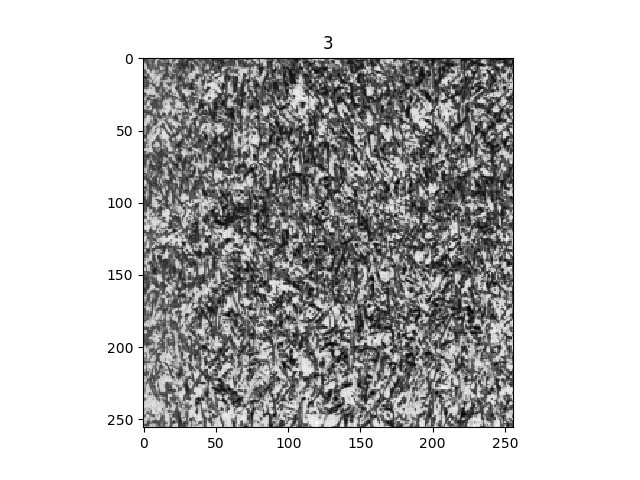
\includegraphics[width=5.5cm]{3.png} }}%
    \qquad
    \subfloat[Histogram of Texture 3]{{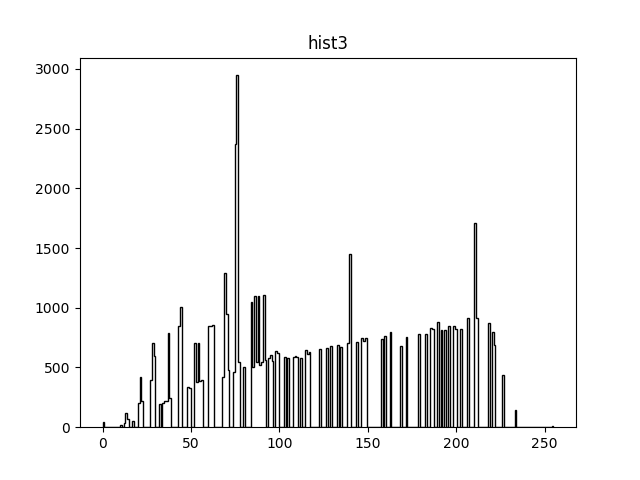
\includegraphics[width=5.5cm]{hist3.png} }}%
    \caption{Texture with histogram}%
    \label{fig:IMG3}%
\end{figure}









\newpage
\subsection{Texture 4}
\textbf{Characteristics:}\\
This texture has a clear pattern of diagonal lines. The lines are a couple of pixels wide, but almost to thin to make a continuous line.(Almost a zigzag pattern instead)  
\\

\textbf{Texture Direction}\\
We have two clear directions in this texture: $\frac{3\pi}{4}$ and $\frac{\pi}{4}$ rads.
\\ 
 
\textbf{Frequency} \\
Frequency of the pattern is 1/3 since the repeating pattern appears three times. 
\\

\textbf{Variance}\\
Compared to the high variance textures, the texture has a lower variance.
\\

\textbf{Homogeneity}\\
There are not any areas with the same px value over a large area, so there are not much of homogeneous areas.  
\\

\textbf{Texture element size}\\
If you think of the texture as the diagonal lines, the size is 3-4 px in width  and 1/6 of the img in length.
\\

\begin{figure}[h]%
	\centering
    \subfloat[Texture 4]{{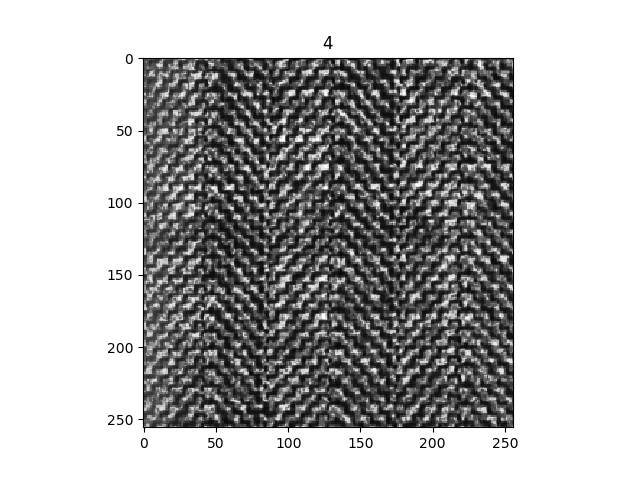
\includegraphics[width=5.5cm]{4.png} }}%
    \qquad
    \subfloat[Histogram of Texture 4]{{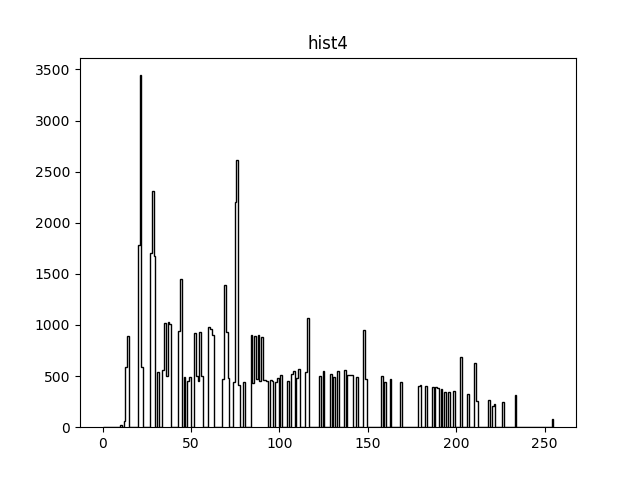
\includegraphics[width=5.5cm]{hist4.png} }}%
    \caption{Texture with histogram}%
    \label{fig:IMG4}%
\end{figure}





\newpage
\subsection{Texture 5}
\textbf{Characteristics:}\\
Another Texture with a clear texture elements consisting of \textit{blocks} that has a regular pattern thought-out the texture.
\\

\textbf{Texture Direction}\\
We have two clear directions in this texture: horizontal and vertical. And like in \ref{fig:IMG1} the texture is skewed of by a couple of degrees.
\\ 
 
\textbf{Frequency} \\
The texture elements are repeating 12-14 times throughout the texture in the horizontal direction, so the horizontal frequency is 1/12. In the same way, the vertical frequency is 1/50. 
\\

\textbf{Variance}\\
This texture has a high variance.
\\

\textbf{Homogeneity}\\
Inside the texture elements we find some homogeneous areas.
\\

\textbf{Texture element size}\\
Texture element size here is the size of the rectangles. The texture element size is 5*20px**2 
\\

\begin{figure}[h]%
	\centering
    \subfloat[Texture 5]{{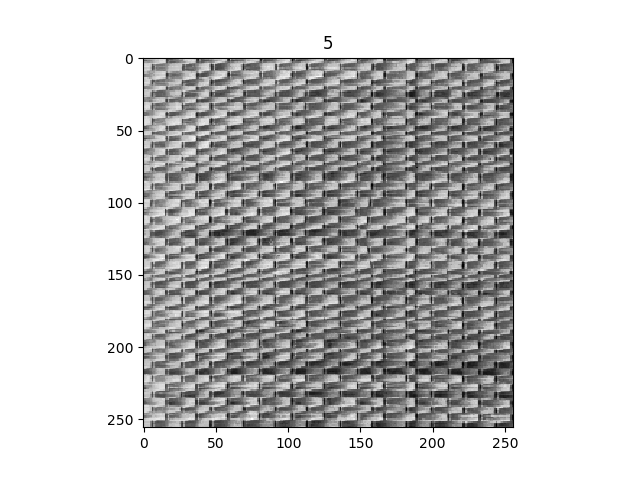
\includegraphics[width=5.5cm]{5.png} }}%
    \qquad
    \subfloat[Histogram of Texture 5]{{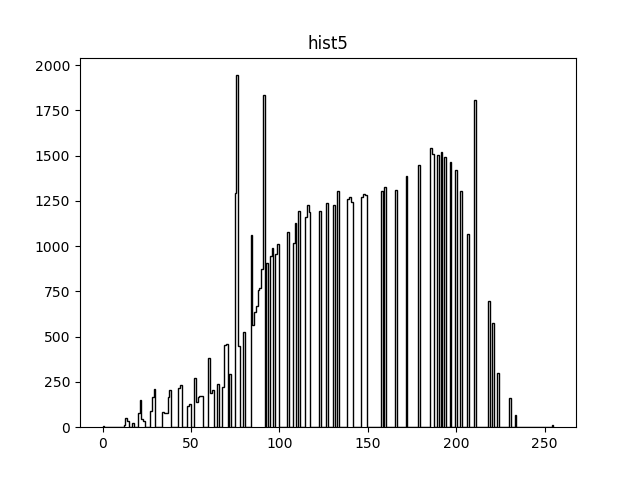
\includegraphics[width=5.5cm]{hist5.png} }}%
    \caption{Texture with histogram}%
    \label{fig:IMG5}%
\end{figure}





\newpage
\subsection{Texture 6}
\textbf{Characteristics:}\\
The texture has clear vertical lines that has a slight counter clockwise angle. 
\\

\textbf{Texture Direction}\\
The texture has an angle if $\frac{\pi}{2}+\epsilon$  
\\ 
 
\textbf{Frequency} \\
The vertical frequency is 1/50 for the whole image.
\\

\textbf{Variance}\\
This texture has a pretty similar variance to \ref{fig:IMG4}.
\\

\textbf{Homogeneity}\\
We find some homogeneous areas if we follow the texture elements in the vertical direction.
\\

\textbf{Texture element size}\\
Texture element size here is 3*250 px**2
\\

\begin{figure}[h]%
	\centering
    \subfloat[Texture 6]{{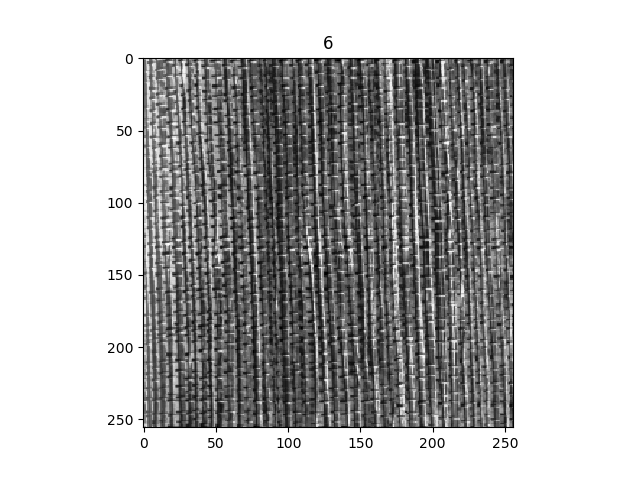
\includegraphics[width=5.5cm]{6.png} }}%
    \qquad
    \subfloat[Histogram of Texture 6]{{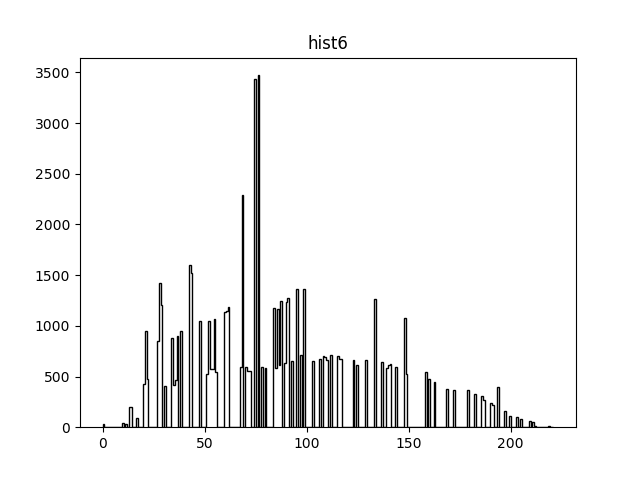
\includegraphics[width=5.5cm]{hist6.png} }}%
    \caption{Texture with histogram}%
    \label{fig:IMG6}%
\end{figure}




\newpage
\subsection{Texture 7}
\textbf{Characteristics:}\\
The characteristics of this texture is pretty similar to \ref{fig:IMG0}.
The texture does not have the same holes as the first one, but if we look at the edges of the image,\ref{fig:ING17CANNY} ,here using canny edge detecting, we see a pretty similar result. 
\\

\textbf{Texture Direction}\\
You can imagine that the texture has an angle if $\frac{3\pi}{4}$ or $\frac{\pi}{4}$, but i would call it isotropic. 
\\ 
 
\textbf{Frequency} \\
Texture frequency is the same as in \ref{fig:IMG1}. approx 3/250. 
\\

\textbf{Variance}\\
This texture has a pretty similar variance to \ref{fig:IMG1}.
\\

\textbf{Homogeneity}\\
We have very few large homogeneous areas. We do have a lot of small ones.
\\

\textbf{Texture element size}\\
Texture element size here is 3*3 px** 2
\\

\begin{figure}[h]%
	\centering
    \subfloat[Texture 7]{{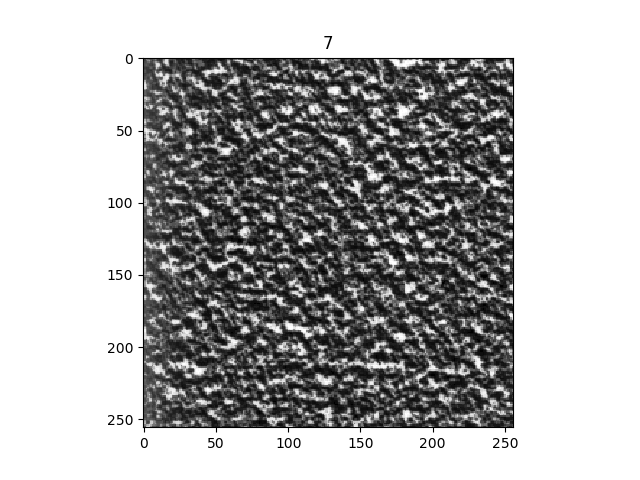
\includegraphics[width=5.5cm]{7.png} }}%
    \qquad
    \subfloat[Histogram of Texture 7]{{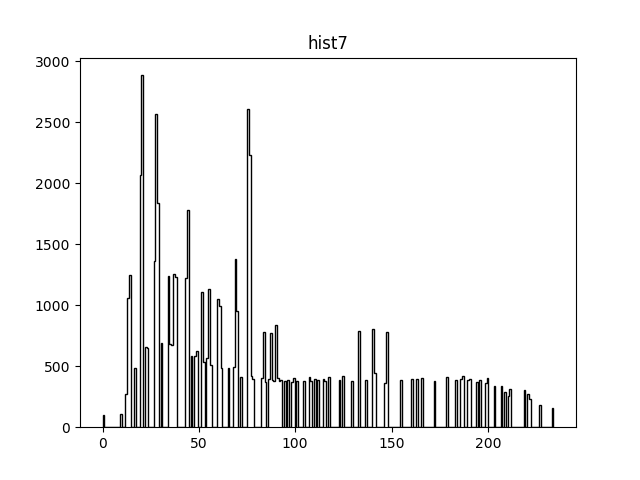
\includegraphics[width=5.5cm]{hist7.png} }}%
    \caption{Texture with histogram}%
    \label{fig:IMG7}%
\end{figure}

\newpage

\begin{figure}[h]%
	\centering
    \subfloat[Canny 0]{{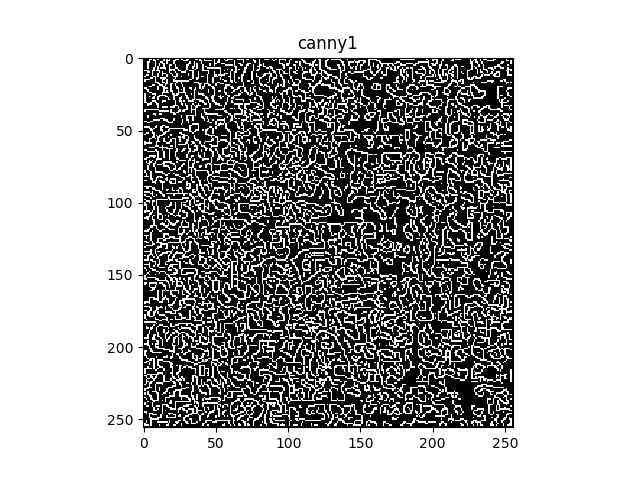
\includegraphics[width=5.5cm]{canny1.png} }}%
    \qquad
    \subfloat[Canny 7]{{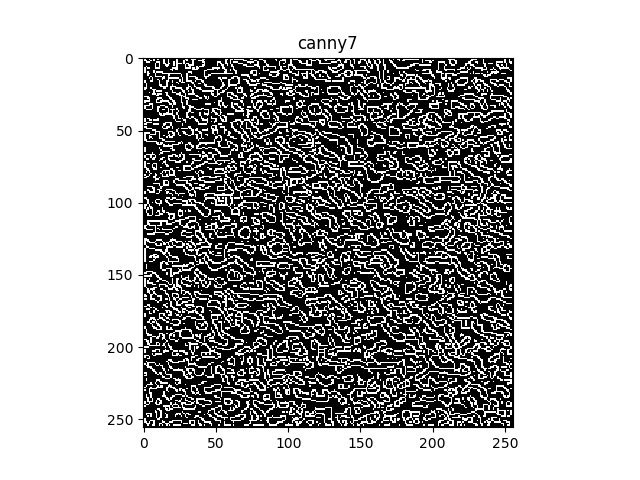
\includegraphics[width=5.5cm]{canny7.png} }}%
    \caption{Comparison of the edges of \ref{fig:IMG0} and \ref{fig:IMG7}}%
    \label{fig:ING17CANNY}%
\end{figure}



\newpage

\section{Visualizing the GLCM matrices}

Now that we have a description of each image we want to work on each one of the images separately. And the first thing we want to do is to find a suitable GLCM.
The problem with running a GLCM on the images is that we have 255 different grey-levels. So there are two operations we want to do before we continue.\\
\begin{itemize}
	\item rescale the histogram\footnote{The reason that we rescale the histogram is to ensure that the histogram isn't skewed. With a rescaled histogram we can be more certain that the GLCM is better represented.}
	\item reduce the number of grey levels.
\end{itemize}    

This can be done with the cv2 and skimage packages:
\begin{lstlisting}[language=python]

equalized_hist=cv2.equalizeHist(original_img)

equalized_rescaled_hist=(ski.exposure.rescale_intensity(equalized_hist, out_range=(0, 15)))
\end{lstlisting}

At the end we get the Original picture histeq-ed with 16 grey-levels. 

\begin{figure}[h]%
	\centering
    \subfloat[Old Histogram]{{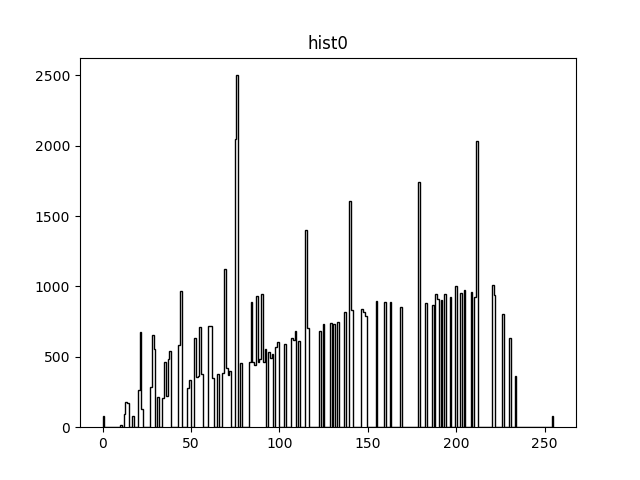
\includegraphics[width=5.5cm]{hist0.png} }}%
    \qquad
    \subfloat[New Histogram]{{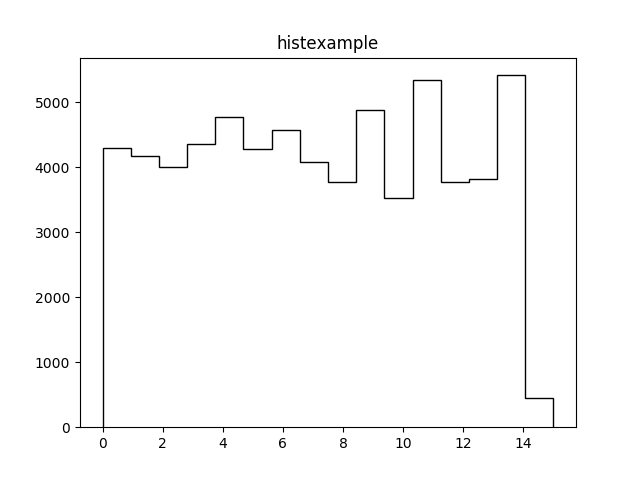
\includegraphics[width=5.5cm]{histexample.png} }}%
    \caption{Transformation of the histogram (just an example, not actual transformation)}%
    \label{fig:Transform}%
\end{figure}


\newpage
\subsection{The GLCM vals}
	\setcounter{subsubsection}{-1}	
	\subsubsection{Texture 0}
		As we remember from \ref{fig:IMG0} we should use the angle $\frac{3\pi}{4}$ and the dist 4px.\\
	\subsubsection{Texture 1}
		As we remember from \ref{fig:IMG1} we should use the angle 0 and angle $\pi$ rad the dist 4px.\\
	\subsubsection{Texture 2}
		As we remember from \ref{fig:IMG2} we should use the angle $1.745$ rad and the dist 8 px. (length can vary on this one)\\
	\subsubsection{Texture 3}
		As we remember from \ref{fig:IMG3} it was isotropic , so we use dist 2px. (isotropic is here just the average of linspace(0,$2\pi$,4))\\
	\subsubsection{Texture 4}
		As we remember from \ref{fig:IMG4} we should use the angle $\frac{3\pi}{4}$ and the angle $\frac{\pi}{4}$ the dist 7px.\\
	\subsubsection{Texture 5}
		As we remember from \ref{fig:IMG5} we should use the angle 0 rad and angle $\pi$ rad the dist 4 and 12 respectively\\
	\subsubsection{Texture 6}
		As we remember from \ref{fig:IMG6} we should use the angle $\pi$ and the dist 8px (here we can use any length, preferably something that is not in the frequency of the horizontal component)\\
	\subsubsection{Texture 7}
		As we remember from \ref{fig:IMG7} it was isotropic , so we use dist 3px. (isotropic is here just the average of linspace(0,$2\pi$,4))\\

\subsection{The GLCM Results}
	\setcounter{subsubsection}{-1}
	\textit{Keep in mind that the normalization of the textures often cut out most of the highest values, so it looks like we have no 15 value pixels. In truth they do exist, but we have only a few of them.}	
	\subsubsection{Texture 0}
		\begin{figure}[h]%
			\centering
    		\subfloat[GCLM 0 0]{{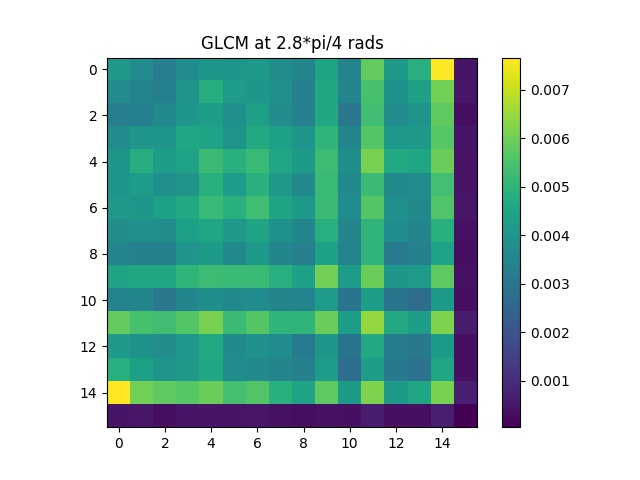
\includegraphics[width=5.5cm]{GCLM_IMG_0_0.jpg} }}%
    		\qquad
    		\subfloat[GCLM 0 1]{{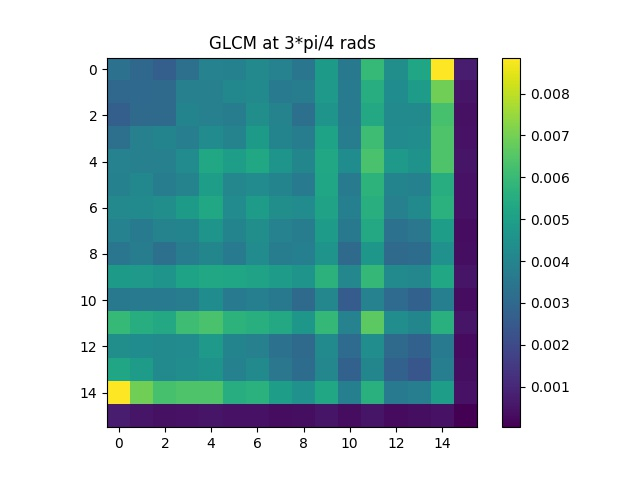
\includegraphics[width=5.5cm]{GCLM_IMG_0_1.jpg} }}%
    		\qquad
    		\subfloat[GCLM 0 2]{{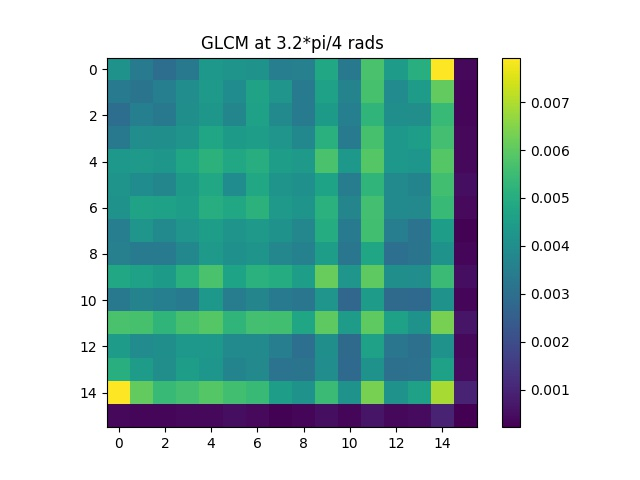
\includegraphics[width=5.5cm]{GCLM_IMG_0_2.jpg} }}%
    		\qquad
    		\subfloat[Texture 0]{{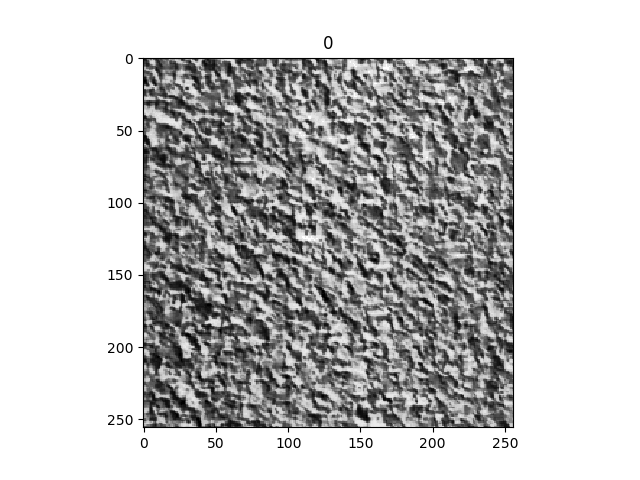
\includegraphics[width=5.5cm]{0.png} }}%
    		\caption{GLCM IMG 0: pi rad}%
    		\label{fig:GLCM_0}%
		\end{figure}
		As we can see from the GLCM of the first picture, we got a lot of pixels switching between 0 and 14 in all 3 of the tests. This could indicate that we have a pattern, but it is more likely that any angle would produce this result. 
\newpage		
	\subsubsection{Texture 1}
		\begin{figure}[h]%
			\centering
    		\subfloat[GCLM 1 0]{{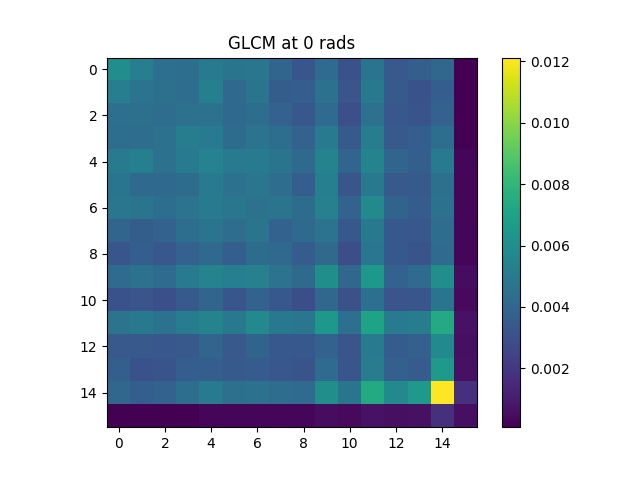
\includegraphics[width=5.5cm]{GCLM_IMG_1_0.jpg} }}%
    		\qquad
    		\subfloat[GCLM 1 1]{{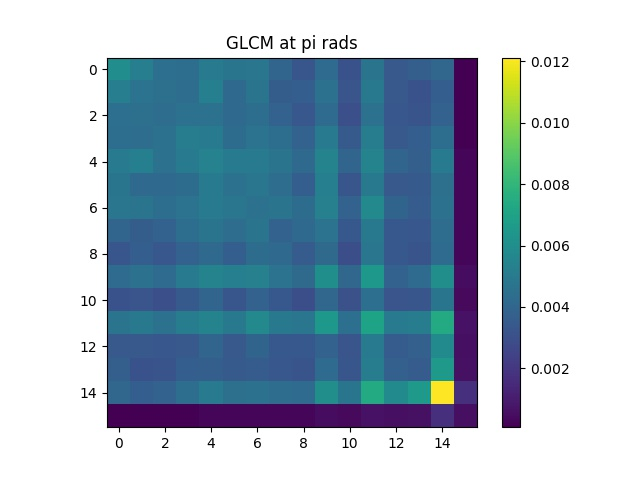
\includegraphics[width=5.5cm]{GCLM_IMG_1_1.jpg} }}%
    		\qquad
    		\subfloat[GCLM 1 2]{{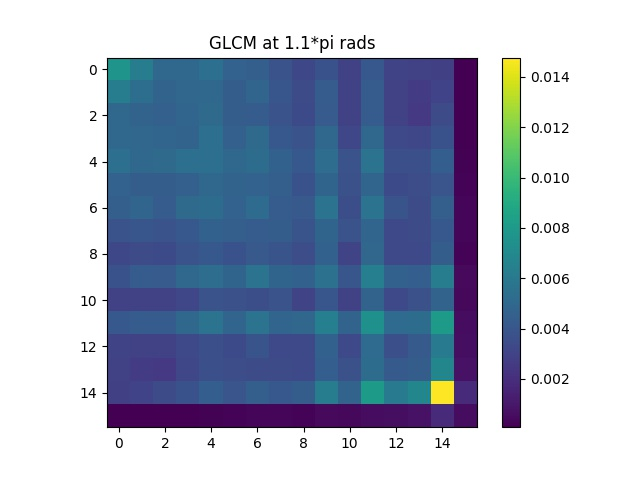
\includegraphics[width=5.5cm]{GCLM_IMG_1_2.jpg} }}%
    		\qquad
    		\subfloat[Texture 1]{{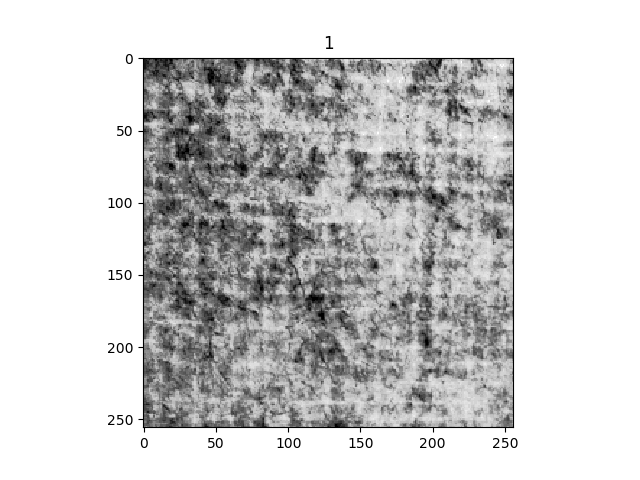
\includegraphics[width=5.5cm]{1.png} }}%
    		
    		\caption{GLCM IMG 1: pi rad}%
    		\label{fig:GLCM_1}%
		\end{figure}
		Again we have pretty similar result in all 3 tests. I don't think we can draw any clear results from this test.
\newpage
	\subsubsection{Texture 2}
		\begin{figure}[h]%
			\centering
    		\subfloat[GCLM 2 0]{{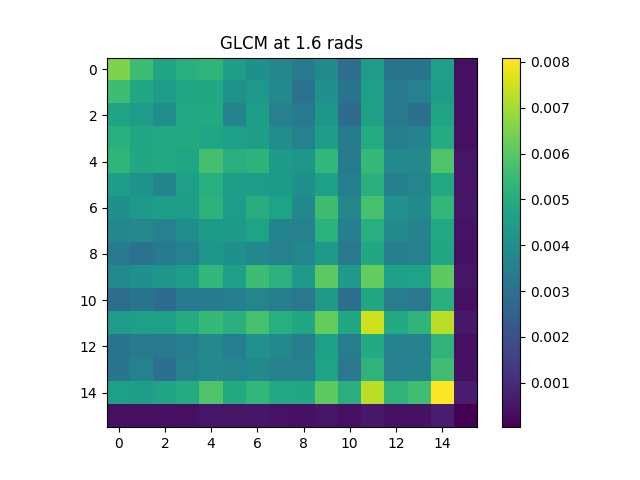
\includegraphics[width=5.5cm]{GCLM_IMG_2_0.jpg} }}%
    		\qquad
    		\subfloat[GCLM 2 1]{{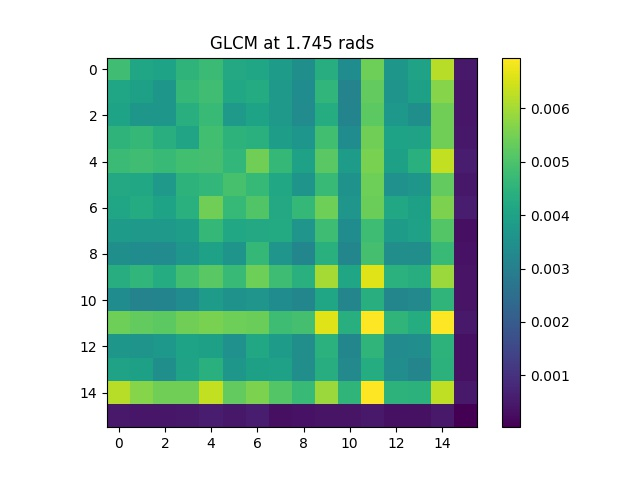
\includegraphics[width=5.5cm]{GCLM_IMG_2_1.jpg} }}%
    		\qquad
    		\subfloat[GCLM 2 2]{{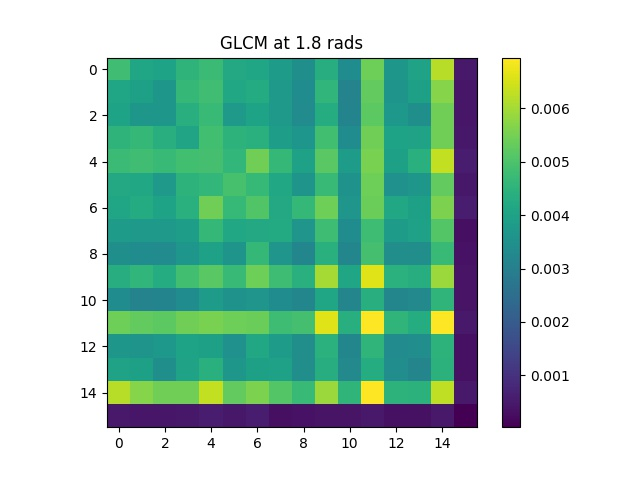
\includegraphics[width=5.5cm]{GCLM_IMG_2_2.jpg} }}%
    		\qquad
    		\subfloat[Texture 2]{{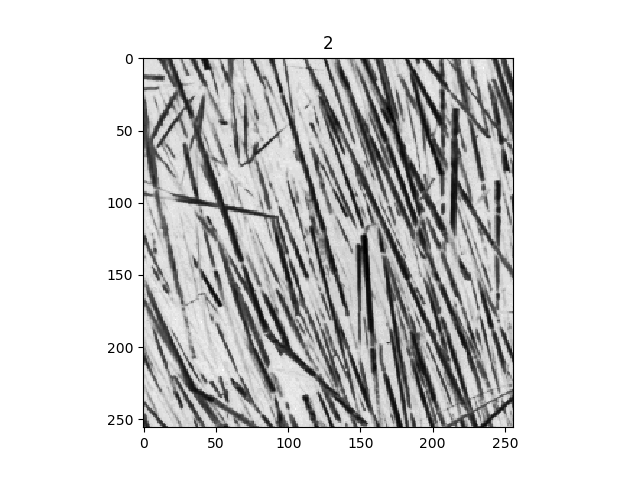
\includegraphics[width=5.5cm]{2.png} }}%

    		\caption{GLCM IMG 2: pi rad}%
    		\label{fig:GLCM_2}%
		\end{figure}
		Here we have tried to land on the same line twice. From the tests, it looks like we had some good results at b) and c), since we have some good jumps from high values to other high values.
\newpage
	\subsubsection{Texture 3}
		\begin{figure}[h]%
			\centering
    		\subfloat[GCLM 3 0]{{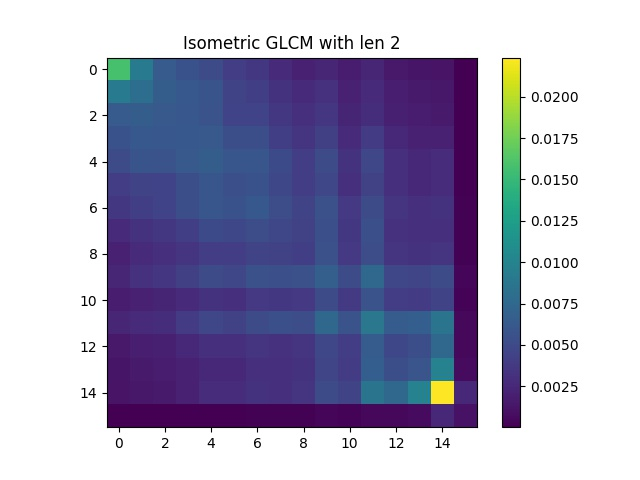
\includegraphics[width=5.5cm]{GCLM_IMG_3_0.jpg} }}%
    		\qquad
    		\subfloat[GCLM 3 1]{{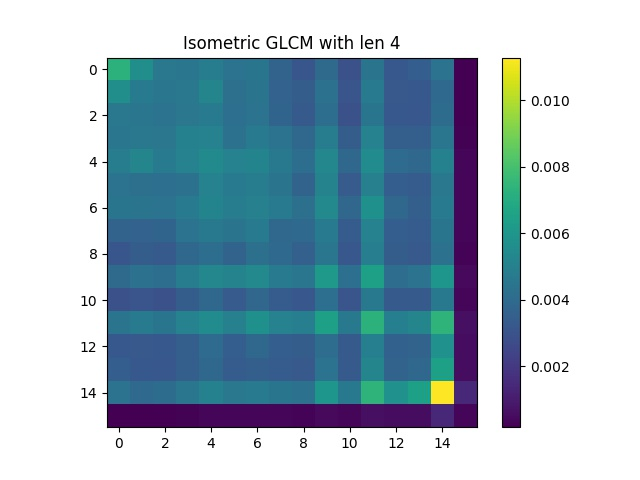
\includegraphics[width=5.5cm]{GCLM_IMG_3_1.jpg} }}%
    		\qquad
    		\subfloat[GCLM 3 2]{{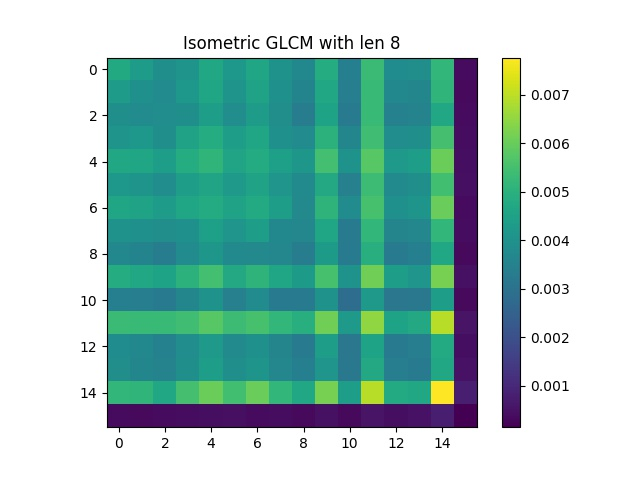
\includegraphics[width=5.5cm]{GCLM_IMG_3_2.jpg} }}%
    		\qquad
    		\subfloat[Texture 3]{{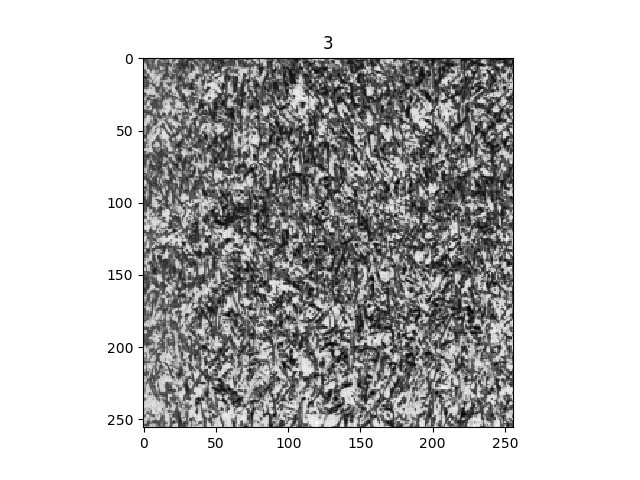
\includegraphics[width=5.5cm]{3.png} }}%

    		\caption{GLCM IMG 3: pi rad}%
    		\label{fig:GLCM_3}%
		\end{figure}
		Number 3 was an isometric test, so we are here looking at the length, and not the angle if the GLCM input. (a) gives us the best result, where we can clearly see that we either stay at a high value, or we stay at a low value.
\newpage
	\subsubsection{Texture 4}
		\begin{figure}[h]%
			\centering
    		\subfloat[GCLM 4 0]{{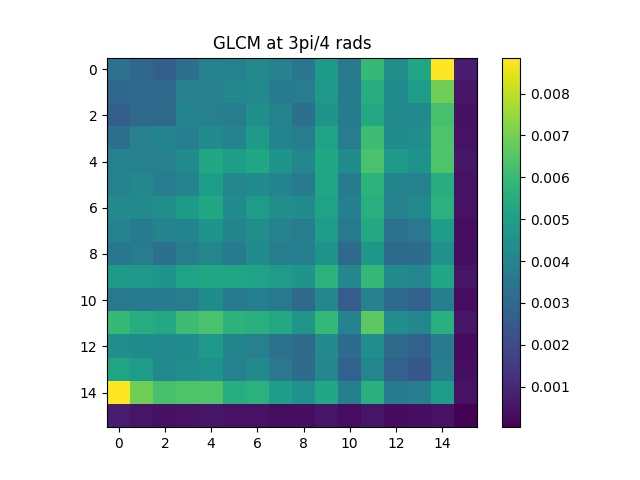
\includegraphics[width=5.5cm]{GCLM_IMG_4_0.jpg} }}%
    		\qquad
    		\subfloat[GCLM 4 1]{{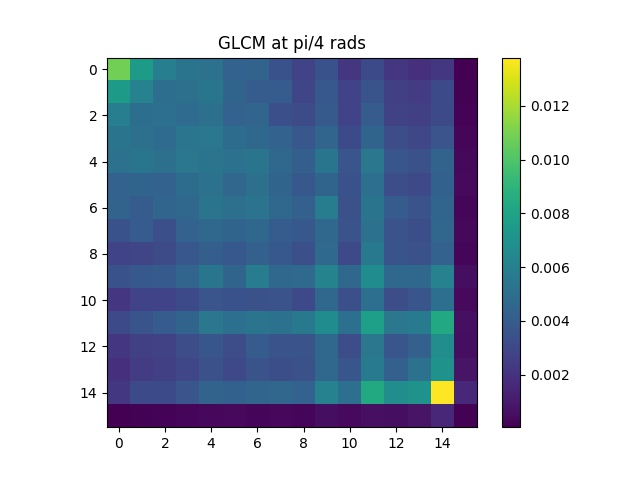
\includegraphics[width=5.5cm]{GCLM_IMG_4_1.jpg} }}%
    		\qquad
    		\subfloat[GCLM 4 2]{{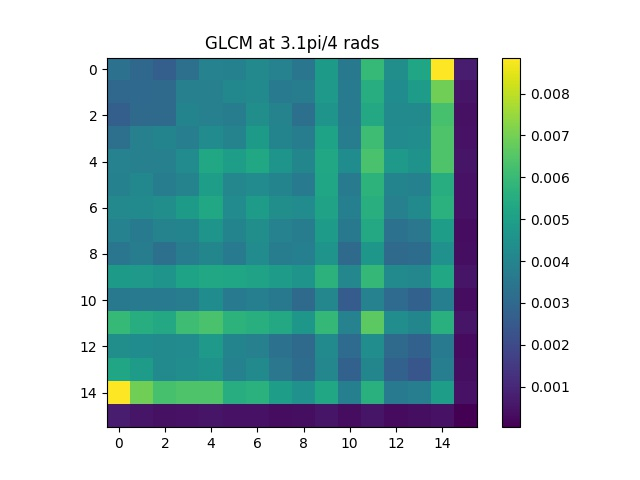
\includegraphics[width=5.5cm]{GCLM_IMG_4_2.jpg} }}%
    		\qquad
    		\subfloat[Texture 4]{{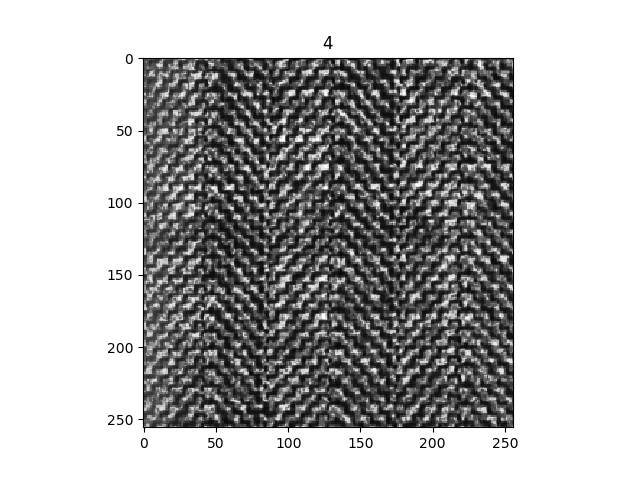
\includegraphics[width=5.5cm]{4.png} }}%

    		\caption{GLCM IMG 4: pi rad}%
    		\label{fig:GLCM_4}%
		\end{figure}
		We are here looking at a diagonal GLCM, and especially (b) yields a good result. It looks like we have a texture pattern.		
		
\newpage
	\subsubsection{Texture 5}
		\begin{figure}[h]%
			\centering
    		\subfloat[GCLM 5 0]{{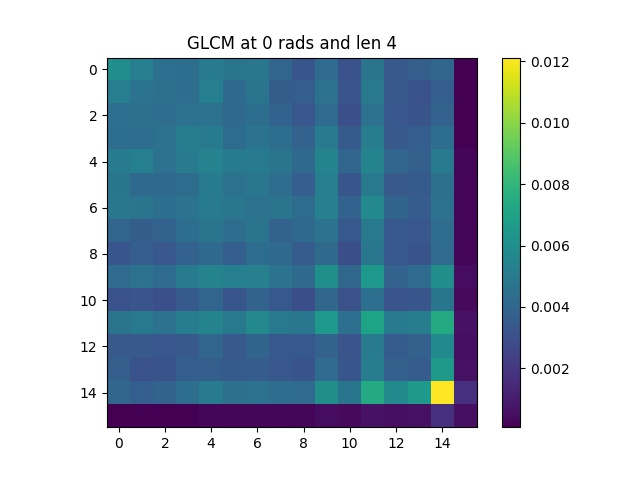
\includegraphics[width=5.5cm]{GCLM_IMG_5_0.jpg} }}%
    		\qquad
    		\subfloat[GCLM 5 1]{{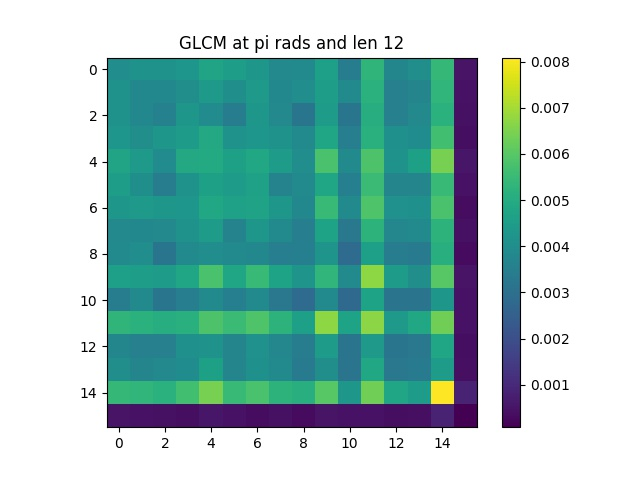
\includegraphics[width=5.5cm]{GCLM_IMG_5_1.jpg} }}%
    		\qquad
    		\subfloat[GCLM 5 2]{{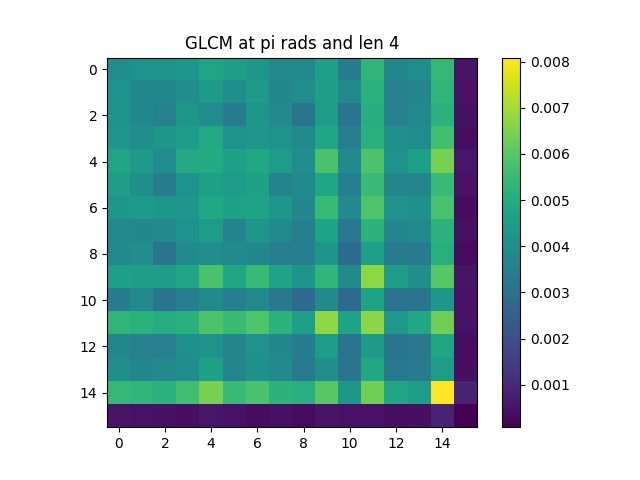
\includegraphics[width=5.5cm]{GCLM_IMG_5_2.jpg} }}%
    		    		\qquad
    		\subfloat[Texture 5]{{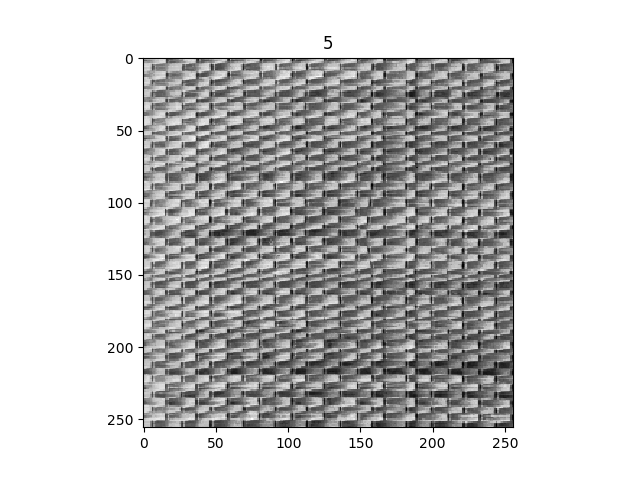
\includegraphics[width=5.5cm]{5.png} }}%

    		\caption{GLCM IMG 5: pi rad}%
    		\label{fig:GLCM_5}%
		\end{figure}
		Texture 5 gave us the best result in (a)
	
\newpage
	\subsubsection{Texture 6}
		\begin{figure}[h]%
			\centering
    		\subfloat[GCLM 6 0]{{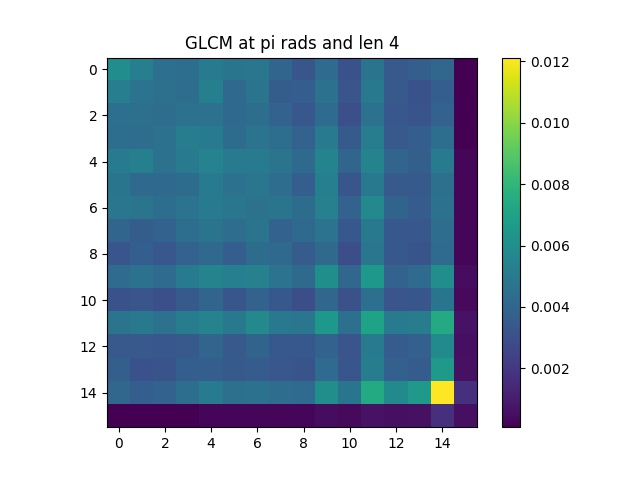
\includegraphics[width=5.5cm]{GCLM_IMG_6_0.jpg} }}%
    		\qquad
    		\subfloat[GCLM 6 1]{{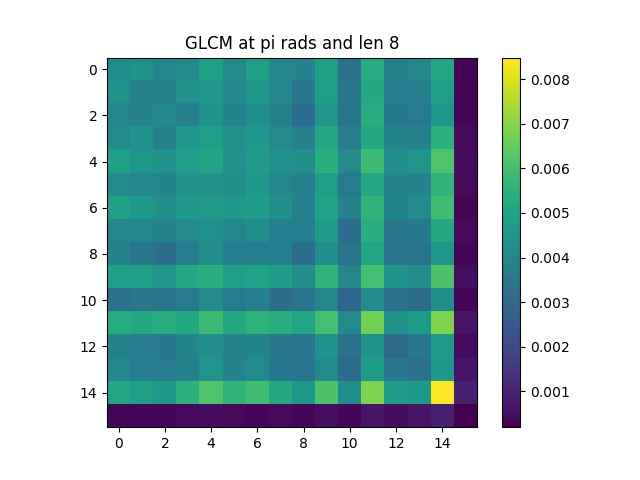
\includegraphics[width=5.5cm]{GCLM_IMG_6_1.jpg} }}%
    		\qquad
    		\subfloat[GCLM 6 2]{{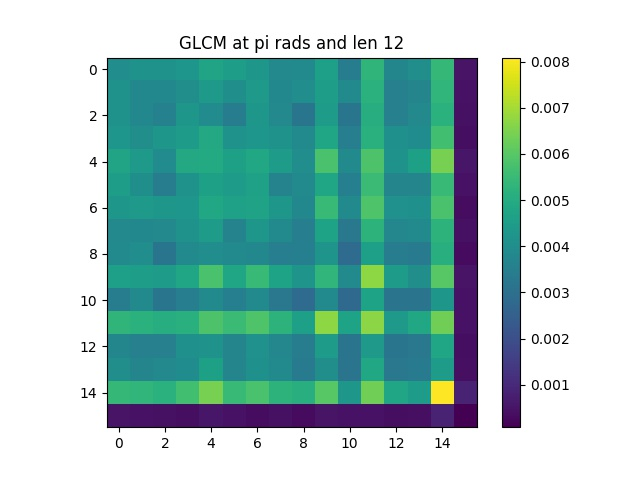
\includegraphics[width=5.5cm]{GCLM_IMG_6_2.jpg} }}%
    		    		\qquad
    		\subfloat[Texture 6]{{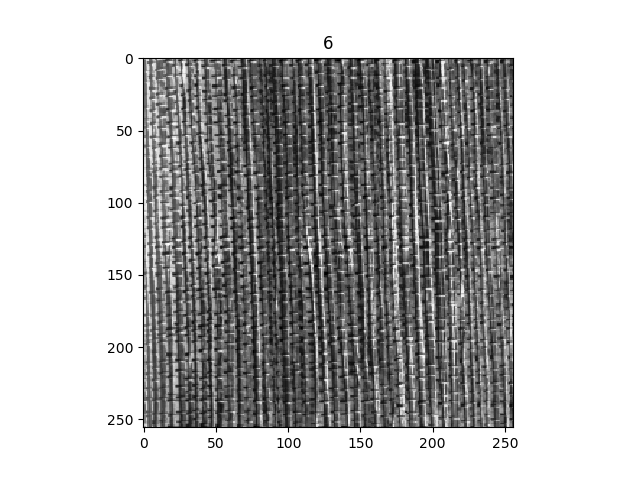
\includegraphics[width=5.5cm]{6.png} }}%

    		\caption{GLCM IMG 6: pi rad}%
    		\label{fig:GLCM_6}%
		\end{figure}
		At texture 6 we got the best result at (a), this is because of the short length. It is less likely to swey off target compared to the other length.		
		
\newpage
	\subsubsection{Texture 7}
		\begin{figure}[h]%
			\centering
    		\subfloat[GCLM 7 0]{{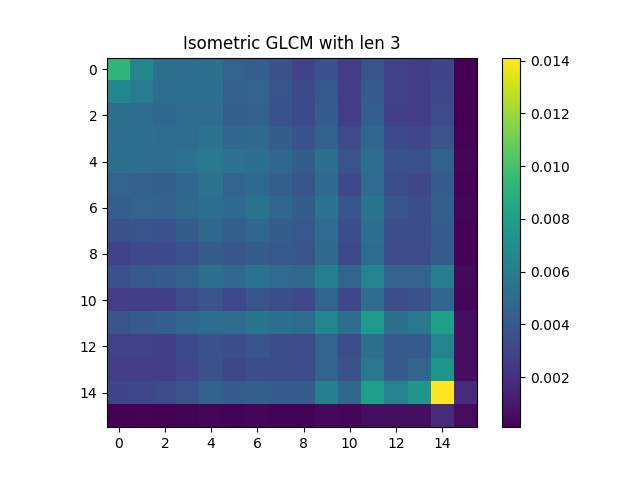
\includegraphics[width=5.5cm]{GCLM_IMG_7_0.jpg} }}%
    		\qquad
    		\subfloat[GCLM 7 1]{{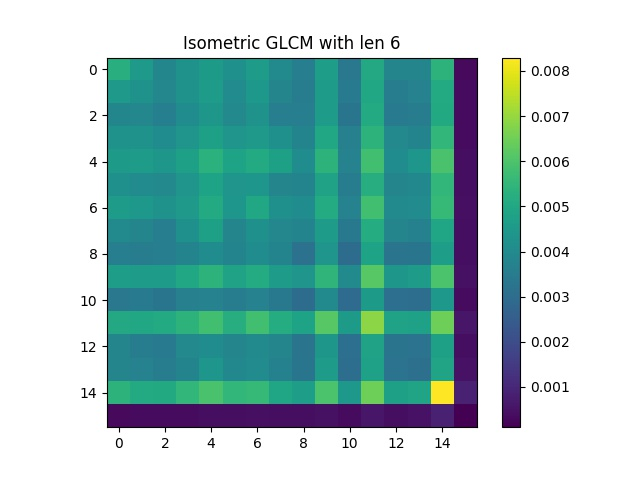
\includegraphics[width=5.5cm]{GCLM_IMG_7_1.jpg} }}%
    		\qquad
    		\subfloat[GCLM 7 2]{{\includegraphics[width=5.5cm]{GCLM_IMG_7_2.jpg} }}%
    		    		\qquad
    		\subfloat[Texture 7]{{\includegraphics[width=5.5cm]{7.png} }}%

    		\caption{GLCM IMG 7: pi rad}%
    		\label{fig:GLCM_7}%
		\end{figure}
		Texture 7 is another isometric GLCM, and the shortest length gave us the best result.

\section{Computing features}
	Now that we have the have the GLCM matrices, we can now try to find:
	\begin{itemize}
		\item GLCM homogeneity
		\item GLCM inertia
		\item GLCM cluster shade
	\end{itemize}
	The formulas for the sliding window is in the assignment, and the code for the sliding window is found in appendix A.
\newpage
\subsection{Computing features result}
	\begin{figure}[h]%
		\centering
    	\subfloat[First 4 inertia images]{{\includegraphics[width=5.5cm]{oppg4inertia0.png} }}%
	    \qquad
	    \subfloat[Last 4 inertia images]{{\includegraphics[width=5.5cm]{oppg4inertia1.png} }}%
	    \caption{Global inertia with sliding window with size 25}%
    	\label{fig:INERTIA}%
\end{figure}
Here we can see the global inertia, with a windowsize of 25. I've used the value 25 for the window size for all 3 of the calculations. This is because it is big enough to get multiple texture elements, and also small enough to not take multiple textures at once.   
	\begin{figure}[h]%
		\centering
    	\subfloat[First 4 homogeneity images]{{\includegraphics[width=5.5cm]{oppg4homo0.png} }}%
	    \qquad
	    \subfloat[Last 4 homogeneity images]{{\includegraphics[width=5.5cm]{oppg4homo1.png} }}%
	    \caption{Global homogeneity with sliding window with size 25}%
    	\label{fig:homo}%
\end{figure}



\begin{figure}[h]%
		\centering
    	\subfloat[First 4 cluster shade images]{{\includegraphics[width=5.5cm]{oppg4cluster0.png} }}%
	    \qquad
	    \subfloat[Last 4 cluster shade images]{{\includegraphics[width=5.5cm]{oppg4cluster1.png} }}%
	    \caption{Global cluster shade with sliding window with size 25}%
    	\label{fig:cluster}%
\end{figure}

\newpage
\section{The GLCM Global thresholding}

	Now that we have the features from assignment C, we can now use the result to try to globally threshold:
\subsection{Inertia}


From \ref{fig:INERTIA}, we can assume that the first image has a threshold of 5 and the second 8.
		 
		 
\begin{figure}[h]%
		\centering
    	\subfloat[First 4 inertia images]{{\includegraphics[width=5.5cm]{oppg4inertia0filter.png}}}%
	    \qquad
	    \subfloat[Last 4 inertia images]{{\includegraphics[width=5.5cm]{oppg4inertia1filter.png} }}%
	    \caption{filter of the inertia}%
    	\label{fig:inertiafilter}%
\end{figure}	

From this result we managed to filter out one of the textures from each picture.

\newpage 
\section{Homogeneity}

From \ref{fig:homo}, we can assume that the first image has a threshold of 0.45 and the second image 0.5
		 
		 
\begin{figure}[h]%
		\centering
    	\subfloat[First 4 homogeneity images]{{\includegraphics[width=5.5cm]{oppg4homo0filter.png}}}%
	    \qquad
	    \subfloat[Last 4 homogeneity images]{{\includegraphics[width=5.5cm]{oppg4homo1filter.png} }}%
	    \caption{filter of the homogeneity}%
    	\label{fig:homofilter}%
\end{figure}	

From this result we managed to filter out one of the textures from each picture.
	

	 
	 from homogeneity we can se tht the first img has threshold 0.45 and the second 0.5
	 
	 45000 and 60000

\newpage
\subsection{Cluster shade}
	From \ref{fig:cluster}, we can assume that the first image has a threshold of 450000 and the second image 60000
		 
		 
\begin{figure}[h]%
		\centering
    	\subfloat[First 4 cluster shade images]{{\includegraphics[width=5.5cm]{oppg4cluster0filter.png}}}%
	    \qquad
	    \subfloat[Last 4 cluster shade images]{{\includegraphics[width=5.5cm]{oppg4cluster1filter.png} }}%
	    \caption{filter of the cluster shade}%
    	\label{fig:clusterfilter}%
\end{figure}	
\newpage
\subsection{Comment on thresholding}
	In this last assignment, we used the most primitive way of thresholding: trail and error.\\ 
	Another way is to use one of the predetermined algorithms from the course:
\begin{figure}[h]%
		\includegraphics[scale=0.27]{save4.png}
	    \caption{Different algorithms for testing thresholding}
    	\label{fig:otsuandfriends}%
\end{figure}	
This is in the case that you need an automatic way to find the threshold. 
	 
\section{Appendix A}
This is the main program, that runs though all the assignments.
\lstinputlisting[language=Python]{../assignment1.py}

\section{Appendix B}
This is all the functions used by the main program
\lstinputlisting[language=Python]{../funcs.py}

	
\end{document}\\

